\documentclass[a4paper,10pt,twoside]{report}

\usepackage{Packages}

\addto\captionsbritish{\renewcommand{\contentsname}{Tabla de Contenidos}}

%\linenumbers

\newcommand{\shortdoctitle}{Doc title}
\newcommand{\doctitle}{Formalización del problema de la partición del grafo}

\newcommand{\authorone}{Laura Rodríguez Navas \\ rodrigueznavas@posgrado.uimp.es}
\newcommand{\monthYear}{Junio 2020}

\author{\me}

\hypersetup
{
    pdfauthor   = {\authorone},
    pdftitle    = {\shortdoctitle},
    pdfsubject  = {\doctitle}
}

\begin{document}

\begin{titlepage}
\begin{center}

\includegraphics[height=2.1cm]{Figures/uimp-logo.png} \\
\LARGE
Resolución de problemas con metaheurísticos \\
\Large
Informe \\
\large

\vspace*{10cm}

\setlength{\TPHorizModule}{1mm}
\setlength{\TPVertModule}{\TPHorizModule}

\newlength{\backupparindent}
\setlength{\backupparindent}{\parindent}
\setlength{\parindent}{0mm}

\begin{textblock}{155}(32,89)
    \vspace*{1mm}
    \huge
    \textbf{\doctitle \\}
    \Large
    \vspace*{5mm}
    % \textit{\docsubtitle} \\
    \vspace*{5mm}
    \Large
     \begin{tabular}{c c c}
            \authorone
    \end{tabular} \\
\end{textblock}

\vfill
%\docdate \\
\large
\monthYear \\

\setlength{\parindent}{\backupparindent}
\end{center}
\end{titlepage} 

\normalsize

\chapter*{Resumen}\label{chapter:Resumen}
\setcounter{page}{0}
\pagenumbering{arabic}
\addcontentsline{toc}{chapter}{Resumen}
Dentro del amplio campo de la Teoría de Grafos, en este informe se considera el problema de la partición del grafo: dado un grafo no dirigido cuyo número de vértices es par y cuyas aristas tienen asociado un peso, se trata de encontrar la partición del conjunto de vértices en dos subconjuntos de tamaño similar de manera que se minimice la suma de los pesos de aquellas aristas que unen vértices que están en diferentes conjuntos

En el capítulo inicial se presenta una breve introducción y descripción del problema. En el segundo capítulo, se describen tres codificaciones para este problema, señalando sus aspectos más relevantes. Concretamente, las codificaciones son implementaciones en Python de los algoritmos basados en técnicas metaheurísticas: Kernighan-Lin, Spectral Bisection y Multilevel Spectral Bisection. En el tercer capítulo, se hace una comparativa entre las diferentes codificaciones. Finalmente, en el último capítulo se presentan algunas conclusiones.

Las codificaciones que se describen en este informe se encuentran en el repositorio:

\begin{center}
	\url{https://github.com/lrodrin/masterAI/tree/master/A2}\label{GitHub}
\end{center}


\tableofcontents

\chapter{Introducción a la Partición de Grafos}\label{chapter:Introduccion}
\section{Partición de Grafos}

Los grafos son una forma eficiente de representar estructuras de datos complejas y contienen todo tipo de información. Cuando un grafo se acerca o incluso excede los límites de memoria, se vuelve más difícil y muy costoso de procesar si no está particionado. La solución es dividir el grafo de manera que las particiones se puedan cargar en la memoria. Al particionar un grafo, los nodos y las aristas se deben dividir uniformemente para tener un buen equilibrio en la distribución de los recursos. Esto es necesario para mantener la máxima eficiencia.

La partición de grafos es una disciplina ubicada entre las ciencias computacionales y la matemática aplicada. La mayoría del trabajo previo en esta disciplina fue realizada por matemáticos que se enfocaron principalmente en lograr el equilibrio en la distribución de los recursos repartiendo uniformemente estos recursos entre las particiones.

En los últimos años los grafos han sido ampliamente utilizados, en consecuencia, el problema de la partición de grafos también ha sido ampliamente estudiado. El problema de la partición de grafos es un problema muy conocido ya que se deriva de situaciones del mundo real que tiene aplicaciones en muchas áreas. 

La primera aplicación del problema fue en la partición de componentes de un circuito en un conjunto de tarjetas que juntas realizaban tareas en un dispositivo electrónico. Las tarjetas tenían un tamaño limitado, de tal manera que el dispositivo no llegara a ser muy grande, y el número de elementos de cada tarjeta estaba restringido. Si el circuito era demasiado grande podía ser dividido en varias tarjetas las cuales estaban interconectadas, sin embargo, el coste de la interconexión era muy elevado por lo que el número de interconexiones debía ser minimizado.

La aplicación descrita fue presentada en \cite{KernighanLin}, en la cual se define un algoritmo eficiente para encontrar buenas soluciones. En la aplicación, el circuito es asociado a un grafo y las tarjetas como subconjuntos de una partición. Los nodos del grafo son representados por los componentes electrónicos y las aristas forman las interconexiones entre los componentes y las tarjetas.

Los algoritmos de partición de grafos utilizados son a menudo complejos. El uso de tales algoritmos da como resultado un procesamiento computacionalmente intenso del grafo que lleva una cantidad considerable de tiempo. Se pueden utilizar algoritmos menos complejos para reducir este tiempo, a costa de una distribución de los recursos menos equilibrada en las particiones.

El enfoque del informe se centra en la división de grafos en dos partes. Se ha elegido la partición en dos partes porque es la forma más sencilla de comparar las particiones con un método de \textit{"bisection"} (que siempre crea dos particiones). Además, asumiremos que la forma más eficiente de particionar todos los tipos de grafos no se limita a un solo algoritmo de partición. La codificación de tres algoritmos se utiliza para examinar el problema de partición de grafos: Kernighan-Lin, Spectral Bisection y Multilevel Spectral Bisection (ver sección \ref{chapter:Algoritmos}).

Su objetivo se centra en particionar diferentes grafos usando los algoritmos anteriores. Inicialmente se han usado grafos más pequeños para describir los algoritmos de partición y la hora de compararlos se han usado grafos más grandes para probar si el código sigue produciendo computacionalmente buenos resultados.

\section{Descripción del problema de Partición de Grafos}

El problema de partición de grafos puede formularse como un problema de programación lineal. La programación lineal se dedica a maximizar o minimizar (optimizar) una función lineal, denominada función objetivo, de tal forma que las variables de dicha función están sujetas a una serie de restricciones expresadas mediante un sistema de ecuaciones o inecuaciones también lineales. 

\newpage
Concretamente, el problema de partición de grafos puede formularse como un problema de programación lineal entera porqué los pesos de las aristas normalmente toman valores enteros. Los problemas de programación lineal entera generalmente están relacionados directamente con problemas de optimización combinatoria, esto genera que al momento de resolver los problemas de programación lineal entera se encuentren restricciones dado el coste computacional de resolverlos. Por ese motivo los algoritmos que buscan soluciones a este problema no pueden garantizar que la solución encontrada sea la óptima. 

El problema de partición de grafos ha sido denominado como un problema NP-completo\cite{NPCompleteness}, lo que implica que las soluciones para él no pueden ser encontradas en tiempos razonables. Entonces, en lugar de encontrar la solución óptima para el problema, recurriremos a algoritmos que pueden no ofrecer la solución óptima pero que dan una buena solución, al menos la mayor parte del tiempo.

La definición formal del problema tiene como objetivo principal, dividir un grafo en \textit{"k"} subgrafos. La única restricción trascendental para resolver el problema es que tiene que haber un número mínimo y máximo de nodos pertenecientes a cada subgrafo. Todos los subgrafos deben tener incorporados al menos 2 nodos y como máximo el doble de los nodos que podrían existir para cada subgrafo si se divide el grafo total en \textit{"k"} subgrafos con la misma cantidad de nodos. En definitiva, que las aristas que unen los subgrafos pesen lo menos posible y de esa manera poder evitar una cierta \textit{"dependencia trascendental"} entre ellos.

La función objetivo es la que pretende minimizar las aristas que unen a los subgrafos. Para ello se analiza su peso, es decir, se intenta maximizar el peso de las aristas que pertenecen a un subgrafo. Esta función es a la que le incorporamos la restricción comentada anteriormente, el número mínimo y máximo de nodos por subgrafo.

A continuación, planteamos el problema de partición de grafos desde un punto de vista más riguroso.

\begin{mydef}\label{def:grafo}
	Un grafo $G$ es un par ordenado $G = (V, E)$, donde $V$ es un conjunto de vértices y $E$ es un conjunto de aristas.
\end{mydef}

Sea $G = (V, E)$ un grafo formado por un conjunto de $n$ vértices $V$ y un conjunto de $m$ aristas $E$.
Dado el grafo $G$, el problema de partición de grafos busca asignar a cada vértice $v \in V$ un entero $p(v) \in \{1, 2, ..., k\}$ tal que:

\begin{itemize}
	\item $p(v) \neq p(u) \, \forall\{u, v\} \in E$
	\item k es mínimo
\end{itemize}

De las particiones sobre el conjunto de vértices $V$, una solución $S$ es representada por un conjunto de $k$ clases de pesos, $S = \{S_{1}, ... S_{k}\}$. Para que la solución $S$ sea factible, es necesario que se cumplan las siguientes restricciones a la vez que se minimice el número de clases de k:

\begin{equation}
	\displaystyle \bigcup_{i = 1} ^ {k} S_{i} = V
\end{equation}

\begin{equation}
	\displaystyle S_{i} \cap S_{j} = \emptyset \, (1 \leq i \neq j \leq k)
\end{equation}

\begin{equation}
	\displaystyle \forall u, v \in S_{i}, \{u, v\} \notin E \, (1 \leq i \leq k)
\end{equation}

\newpage
Las restricciones (1.1) y (1.2) establecen que la solución $S$ debe ser una partición del conjunto de vértices $V$ , mientras que la restricción (1.3) obliga a que ningún par de vértices adyacentes sean asignados a la misma clase, es decir, que todas las clases de pesos en la solución deben formar conjuntos independientes.




\chapter{Algoritmos basados en metaheurísticas}\label{chapter:Algoritmos}
Debido a la \textit{"intratabilidad"} del problema de la partición de grafos, como hemos comentado, no existe un algoritmo concreto que permita obtener en tiempo polinómico una solución óptima a la partición de cualquier grafo. Es por ello por lo que, los algoritmos codificados para este informe se basan en la metaheurística, con el objetivo de obtener soluciones de buena calidad en tiempos computacionales aceptables, a pesar de que los algoritmos metaheurísticos no garantizan que se vaya a obtener una solución óptima al problema.

En el siguiente apartado se describen los algoritmos Kernighan-Lin\cite{KernighanLin} (ver apartado \ref{Kernighan-Lin}), Specrtal Bisection (ver apartado \ref{Spectral-Bisection}) y Multilevel Spectral Bisection (ver apartado \ref{Multilevel-Spectral-Bisection}). Tres algoritmos que se diseñaron específicamente para la resolución del problema de la partición de grafos. Cualquiera de estos algoritmos proporciona una solución factible al problema, pudiendo ser esta óptima o no. El enfoque del informe radica en la partición de diferentes grafos en dos particiones usando estos tres algoritmos. 

Además de describir cada uno de los algoritmos, también se describirán algunos detalles sobre su codificación.
De ejemplo para describir cada codificación se ha utilizado un grafo inicial (ver Figura \ref{grafo}). Este grafo es un grafo no dirigido (ver Definición \ref{no_dirigido}) de diez nodos con pesos en sus aristas.

\begin{mydef}\label{no_dirigido}
	Un grafo no dirigido es un grafo (ver Definición \ref{def:grafo} ) donde: $V\neq \emptyset$ y $E\subseteq \{x\in \mathcal P(V):|x|=2\}$ es un conjunto de pares no ordenados de elementos de $V$. Un par no ordenado es un conjunto de la forma \{a , b\}, de manera que \{a, b\} = \{b, a\}. En los grafos, los conjuntos de pares no ordenados pertenecen al conjunto potencial de $V$, denotado $\mathcal P(V)$, y son de cardinalidad 2. 
\end{mydef}

\renewcommand{\figurename}{Figura}
\begin{figure}[h]
	\centering
	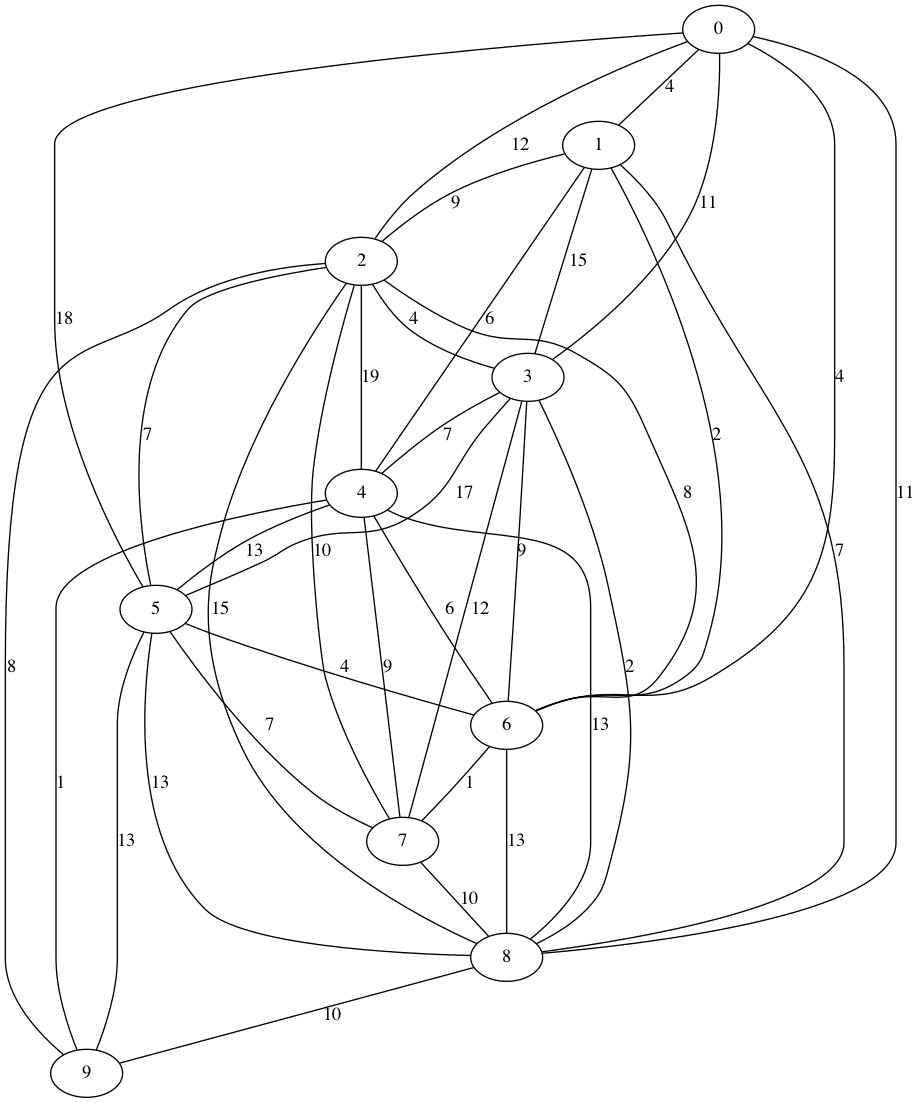
\includegraphics[scale=0.25]{Figures/10_dataset}
	\vspace{1mm}
	\caption{Grafo inicial.}
	\label{grafo}
\end{figure}

\newpage
\section{Kernighan-Lin}\label{Kernighan-Lin}

El algoritmo Kernighan-Lin\cite{KernighanLin}, a menudo abreviado como K-L, es uno de los primeros algoritmos de partición de grafos y fue desarrollado originalmente para optimizar la colocación de circuitos electrónicos en tarjetas de circuito impreso para minimizar el número de conexiones entre las tarjetas (circuitos VLSI\cite{KernighanLin}\cite{Ravikumar}).

El algoritmo es:

\begin{itemize}
	\setlength{\parskip}{0pt}
	\setlength{\itemsep}{0pt plus 1pt}
	\item \textbf{Iterativo}. Porque el grafo inicialmente ya está particionado, pero la aplicación del algoritmo intentará mejorar u optimizar la partición inicial. 
	\item \textbf{Voraz}. Porque el algoritmo hará cambios si hay un beneficio inmediato sin considerar otras formas posibles de obtener una solución óptima. Para ello, elige la opción óptima en cada paso con la esperanza de llegar a una solución general óptima.
	\item \textbf{Determinista}. Porque se obtendrá el mismo resultado cada vez que se aplique el algoritmo. 
\end{itemize}

El algoritmo K-L, como acabamos de describir, no crea particiones, sino que las mejora iterativamente. La idea original era tomar una partición aleatoria y aplicarle Kernighan-Lin\cite{KernighanLin}. Esto se repetiría varias veces y se elegiría el mejor resultado. Mientras que para grafos pequeños esto ofrece resultados razonables, es bastante ineficiente para tamaños de grafos más grandes.

Hoy en día, el algoritmo se usa para mejorar las particiones encontradas por otros algoritmos, tratando de mejorar las particiones mediante el intercambio de nodos vecinos. Por tanto, complementa muy bien otro tipo de algoritmos como por ejemplo los que realizan una partición espectral (ver sección \ref{Spectral-Bisection}).

\subsection{Descripción}

El objetivo del algoritmo es dividir el conjunto de vértices $V$ de un grafo no dirigido (ver Definición \ref{no_dirigido}) en dos subconjuntos disjuntos (ver Definición \ref{disjuntos}) $A$ y $B$ de igual tamaño, de una manera que minimice la suma $T$ de los pesos del subconjunto de aristas que cruzan de $A$ a $B$. El algoritmo mantiene y mejora una partición, en cada iteración usando un algoritmo voraz (ver Definición \ref{voraz}), empareja los vértices de $A$ con los vértices de $B$, de modo que al mover los vértices emparejados de una partición a la otra se maximiza la ganancia, que mide cuánta "información" nos brinda la función objetivo. Después de emparejar los vértices y maximizar la ganancia, crea un subconjunto de los pares de los vértices elegidos para tener el mejor efecto sobre la calidad de la solución $T$. Dado un grafo con n vértices, cada iteración del algoritmo se ejecuta en el tiempo $O({n}^2 \, log \, n)$.

\begin{mydef}\label{disjuntos}
	$A$ y $B$ son dos subconjuntos disjuntos si $A \cup B$ y $A \cap B \neq 0$.
\end{mydef}

\begin{mydef}\label{voraz}
	Dado un conjunto finito $C$, un algoritmo voraz devuelve un conjunto $S$ tal que $S\subseteq C$ y que además cumple con las restricciones del problema inicial. A cada conjunto $S$ que satisfaga las restricciones y que logra que la función objetivo se minimice o maximice (según corresponda) diremos que $S$ es una solución óptima. 
\end{mydef}

Más detalladamente, sea $a$ un elemento del subconjunto $A$ y $b$ un elemento del subconjunto $B$, para cada $a \in A$, $I_{a}$ es el coste interno de a, es decir, la suma de los pesos de las aristas entre a y otros nodos en $A$. Y $E_{a}$ es el coste externo de a, es decir, la suma de los pesos de las aristas entre a y los nodos en $B$. De manera similar, se define $I_{b}$ y $E_{b}$ para cada $b \in B$.

Así podemos decir que existe una diferencia $D$ entre la suma de los costes externos e internos $s$. Si formalizamos obtenemos:

\begin{center}
	$D_{s} = E_{s} - I_{s}$
\end{center}

Y entonces si $a$ y $b$ se intercambian, la ganancia se calcula como:

\begin{center}\label{ganancia}
	$T_{antigua} - T_{nueva} = D_{a} + D_{b} - 2c_{a, b}$ 
\end{center}

donde $c_{a, b}$ es el coste de las aristas posibles entre $a$ y $b$.

El algoritmo intenta encontrar una solución óptima de operaciones de intercambio entre los elementos de $A$ y $B$ que maximice la ganancia ($T_{antigua} - T_{nueva}$) y luego ejecuta las operaciones, produciendo una partición del grafo en $A$ y $B$.

Con estos dos conceptos, podemos describir la primera iteración del algoritmo usando el pseudocódigo en \cite{Ravikumar}.

\begin{lstlisting}[frame=single] 
function Kernighan-Lin(G(V, E)) is
 determine a balanced initial partition of the nodes into sets A and B

 do
  compute D values for all a in A and b in B
  let gv, av, and bv be empty lists
  for n := 1 to |V| / 2 do
    find a from A and b from B, such that gain is maximal
    remove a and b from further consideration in this pass
	add g to gv, a to av, and b to bv
	update D values for the elements of A = A \ a and B = B \ b
  end for
  find k which maximizes g_max, the sum of gv[1], ..., gv[k]
  if g_max > 0 then
    Exchange av[1], av[2], ..., av[k] with bv[1], bv[2], ..., bv[k]
  until (g_max <= 0)  
    
return G(V, E) 
\end{lstlisting}

Entonces, en cada iteración, el algoritmo K-L intercambia pares de vértices para maximizar la ganancia. Y continúa haciéndolo hasta que se intercambian todos los vértices de la partición más pequeña. 

Una gran ventaja del algoritmo es que no se detiene incluso aceptando ganancias negativas, sigue esperando que las ganancias posteriores sean más grandes y que el tamaño de la suma de los pesos de las aristas se reduzca hasta que se intercambian todos los vértices de la partición más pequeña. Esta capacidad es una característica crucial. Aunque esta capacidad sea crucial, el algoritmo tiene unas cuantas desventajas:

\begin{itemize}
	\item Los resultados son aleatorios porque el algoritmo comienza con una partición aleatoria.
	\item Computacionalmente es un algoritmo lento.
	\item Solo se crean dos particiones del mismo tamaño.
	\item Las particiones deben tener el mismo tamaño para que el algoritmo no intente encontrar soluciones óptimas que ya existan.
	\item No resuelve muy bien los problemas con las aristas ponderadas.
	\item La solución dependerá en gran medida de la primera partición.
\end{itemize}

C. Fiduccia y R. Mattheyses realizaron importantes avances prácticos en \cite{FiducciaMattheyses}, quienes mejoraron el algoritmo de  Kernighan-Lin\cite{KernighanLin} de tal manera que, cada partición se ejecuta en $O({n}^2)$, en lugar de $O({n}^2 \, log \, n)$. La reducción se logra en parte eligiendo nodos individuales para intercambiar en lugar de parejas de vértices.

\subsection{Ejemplo de codificación}

Existen muchas variaciones del algoritmo K-L que a menudo intercambian el tiempo de ejecución con la calidad, o generalizan el algoritmo a más de dos particiones. En este caso, para la codificación del algoritmo se ha utilizado la libraría de Python: \href{https://networkx.github.io/documentation/stable/reference/algorithms/generated/networkx.algorithms.community.kernighan_lin.kernighan_lin_bisection.html}{NetworkX}. El algoritmo divide un grafo en dos particiones usando el algoritmo Kernighan-Lin\cite{KernighanLin}. Es decir, divide un grafo en dos conjuntos intercambiando iterativamente pares de nodos para reducir el peso de las aristas entre los dos conjuntos.

\begin{mydef}\label{NetworkX}
	NetworkX es un paquete de Python para la creación, manipulación y estudio de la estructura, dinámica y funciones de los grafos. 
\end{mydef}

Por ejemplo, en una ejecución de la codificación, donde la entrada es el grafo de la Figura \ref{grafo}, y después de una partición inicial, podemos obtener los subconjuntos: A = \{3, 4, 6, 8, 9\} y B = \{0, 1, 2 , 5, 7\}. Estos subconjuntos son del mismo tamaño y sus elementos están ordenados.

En esta ejecución, los pasos que sigue el algoritmo son los siguientes:

\begin{itemize}
	\item Dibuja una línea que separa el grafo en dos particiones con el mismo número de vértices en cada partición.
	\item Cuenta la cantidad de aristas que cruzan la línea. Este número se llama \textit{"cut-size"} y el objetivo es disminuirlo, es decir, disminuir el número de conexiones entre los vértices del grafo.
	\item Encuentra el coste de todos los vértices en el grafo, buscando el número de conexiones que cada vértice tiene dentro de su propia partición y restando eso del número de conexiones que cada vértice tiene con vértices en la otra partición.
	\item Determina la ganancia máxima intercambiando dos nodos. La ecuación de ganancia es la que se muestra en \ref{ganancia}.
	\item Intercambia los dos nodos con la ganancia máxima. Si se han calculado todas las ganancias de emparejamiento de todos los nodos y la ganancia máxima es igual a cero o negativa, los nodos con la ganancia más alta aún deberán intercambiarse.
	\item Resta la ganancia del \textit{"cut-size"} original para obtener el nuevo \textit{"cut-size"}.
	\item Cambia los nodos que se han intercambiado.
	\item Repite estos pasos hasta que la ganancia máxima es cero o negativa.
\end{itemize}

\newpage
\section{Spectral Bisection}\label{Spectral-Bisection}

\subsection{Descripción}

\subsection{Ejemplo de codificación}

Después de la partición obtenemos los conjuntos: A = \{1, 2, 3, 4, 6, 9\} y B = \{0, 8, 5, 7\}.

Los conjuntos no son del mismo tamaño. No están ordenados.

\newpage
\section{Multilevel Spectral Bisection}\label{Multilevel-Spectral-Bisection}

El particionamiento de grafos por multilevel es un método moderno que reduce el tamaño de las particiones del grafo con la combinación de los vértices y las aristas sobre varios niveles, creando particiones del grafo cada vez más pequeñas y extensas con muchas variaciones y combinaciones de diferentes métodos.

\subsection{Descripción}\label{msb_description}

Y esta es, en líneas generales, la descripción de uno de los algoritmos más exitosos para el problema de partición de grafos.

\subsection{Ejemplo de codificación}

El algoritmo Multilevel Spectral Bisection (MSB) descrito en la sección \ref{msb_description} ha resultado ser muy eficiente (ver sección \ref{chapter:Comparativa}). En MSB, se transfiere información aproximada sobre el segundo \textit{eigenvector} del grafo original entre niveles, mejorando esta información en cada nivel y finalmente, se usa otra vez el \textit{eigenvector} para dividir el grafo. 

Se muestra el pseudocódigo del algoritmo a continuación:

\begin{lstlisting}[frame=single] 
Function ML-Partition(G)

  If G is small enough then
    Find partition (V1, V2) of G in some way
    
  else

    Construct a smaller approximation G'
    (V1', V2') = ML-Partition(G')
    (V1", V2") = Project-partition-up (V1', V2')
    (V1, V2)   = Refine-partition (V1", V2")

endif

Return (V1, V2)
\end{lstlisting}

La misma idea se puede usar para dividir el grafo en \textit{p} partes a la vez. En realidad, hay toda una familia de algoritmos que puede dividir grafos en \textit{p} partes a la vez. Algunos de estos algoritmos se encuentran implementados en paquetes de software como Chaco\cite{Chaco}, METIS\cite{MeTis} o WGPP\cite{WGPP}.

Para la codificación del algoritmo se escogió la librería escrita en C de \href{http://glaros.dtc.umn.edu/gkhome/metis/metis/overview}{METIS} junto con NetworkX (ver Definición\ref{NetworkX}). Concretamente, la librería que se ha utilizado de Python es: \href{https://networkx-metis.readthedocs.io/en/latest/reference/generated/nxmetis.partition.html#nxmetis.partition}{NetworkX-METIS}. \textit{NetworkX-METIS} es un complemento para el paquete Python de \textit{NetworkX} que usa METIS\cite{MeTis} para la partición de grafos. Los algoritmos implementados en METIS se basan en los esquemas de bisección multinivel.

Las características clave de METIS son las siguientes:

\begin{itemize}
	\item Proporciona particiones de alta calidad. Los experimentos con una gran cantidad de nodos muestran que METIS produce particiones que son consistentemente mejores que las producidas por otros algoritmos ampliamente utilizados. Las particiones producidas por METIS son consistentemente 10\% a 50\% mejores que las producidas por algoritmos de partición espectral.
	\item Es extremadamente rápido. Los experimentos en una amplia gama de grafos han demostrado que METIS es de uno a dos órdenes de magnitud más rápido que otros algoritmos de partición ampliamente utilizados.
\end{itemize}

METIS es un algoritmo de partición de grafos que se enfoca en minimizar el número de aristas cruzadas de cada partición y distribuir la carga de trabajo de manera uniforme entre las particiones. Con METIS, los gráficos se dividen en tres fases. La primera fase es la fase de engrosamiento, la segunda la fase de partición y la tercera y última fase la fase de no engrosamiento (Figura X). La fase de particionamiento contiene particiones bi-particionadas y K-way. A diferencia de la partición K-way, la bi-partición se realiza de forma recursiva. Las subseccion a continuación contienen una explicación más extensa de estas diversas fases.

Por ejemplo, en una ejecución de la codificación, la entrada es el grafo de la Figura \ref{grafo}. El resultado de aplicar el algoritmo codificado son los conjuntos: A = \{0, 1, 3, 7, 8\} y B = \{2, 4, 5, 6, 9\}. Estos conjuntos tienen el mismo tamaño y sus elementos están ordenados.

\chapter{Comparativa entre los diferentes algoritmos}\label{chapter:Comparativa}
En esta sección, veremos una comparativa entre los algoritmos que hemos descrito en las secciones previas, tras ser aplicados sobre diferentes grafos aleatorios, también conocidos como grafos de Erdös y Renyi\cite{ErdosRenyi} o grafos binomiales. Pero antes de ver la comparativa, en primer lugar, definimos el concepto de grafo aleatorio.

Se dice que un grafo es aleatorio si la presencia y colocación de sus aristas siguen una distribución aleatoria. Por tanto, un grafo aleatorio no puede diseñarse bajo ningún criterio concreto. Los grafos aleatorios también son conocidos como grafos de Erdös y Renyi porqué utilizan el modelo de Erdös y Renyi. El nombre de este modelo proviene de los matemáticos Paul Erdős y Alfréd Rényi, quienes lo presentaron por primera en 1959.

El modelo de Erdös y Renyi (a veces abreviado como modelo ER), es el método que se ha empleado para la generación de los grafos aleatorios de prueba que se usan en la comparativa de las codificaciones. Para ello, los grafos se han construido mediante la conexión de los nodos al azar. Cada arista se incluye en el grafo con una probabilidad de \textit{p} independiente de las otras aristas del grafo. De manera equivalente, todos los grafos con \textit{n} nodos y \textit{m} aristas tienen la misma probabilidad. Esa probabilidad es:

\begin{center}
	$p^m(1 - p)^{{n \choose 2} - m}$
\end{center}

En la implementación de los grafos aleatorios se ha utilizado la librería de Python:  \href{https://networkx.github.io/documentation/latest/reference/generated/networkx.generators.random\_graphs.erdos\_renyi\_graph.html?highlight=erdos\%20renyi#networkx.generators.random\_graphs.erdos\_renyi\_graph}{NetworkX}. Concretamente el método que se ha utilizado nos devuelve un grafo no dirigido, donde se elige cada una de las aristas posibles con probabilidad \textit{p} = 0.7, según el número de nodos de entrada \textit{n}. En particular, el caso \textit{p} = 0.7 se corresponde con el caso en el los \textit{n} vértices se eligen con mayor probabilidad (\textit{p} < 0.5). Los pesos de las aristas también se han generado aleatoriamente dentro de un intervalo de pesos de 1 a 20.

Podemos observar la codificación acabada de describir, que se ejecuta en tiempo $O$($n^2$).

\lstset{language=Python}    
\begin{lstlisting}[frame=single]  
G = nx.erdos_renyi_graph(n, 0.7)

for u, v in G.edges():
  if u != v:
    G[u][v]['label'] = random.randrange(1, 20)
\end{lstlisting}

Y en la tabla siguiente, se presenta una comparación entre los algoritmos codificados sobre los grafos aleatorios generados en este informe, en términos de tiempo computacional. Se muestra el tiempo (en segundos) en completar las ejecuciones de los algoritmos sobre los grafos aleatorios para distintos números de vértices \textit{n}. Para ello se ha utilizado un MacBook Pro, con un procesador de cuatro núcleos de 2.8 GHz y con 16 GB de memoria RAM. Es de esperar que, a mayor número de vértices, los algoritmos tengan mayor tiempo de ejecución.

\renewcommand{\tablename}{Tabla}
\begin{table}[h]	
	\begin{center}
		\begin{tabular}{|c|c|c|c|}
			\hline
			\textit{n} & 307 & 552 & 861 \\
			\hline
			Kernighan-Lin & 0.0117 & 0.0214 & 0.0451\\
			\hline
			Spectral Bisection & 0.0021 & 0.0031 & 0.0060 \\
			\hline
			MSB & 0.0025 & 0.0031 & 0.0037 \\ 
			\hline
		\end{tabular}
		\vspace{1mm}
		\caption{Tabla comparativa de los algoritmos.}
	\end{center}
\end{table}

Podemos ver como los algoritmos Kernighan-Lin, Spectral Bisection y Multilevel Spectral Bisection (MSB) tienen unos tiempos de ejecución similares cuando el número de vértices \textit{n} es más pequeño. Fenómeno que cambia cuando casi se duplican el número de vértices a 552. 

\newpage
Además, si nos fijamos en el algoritmo Kernighan-Lin, cuando el número de vértices casi se duplican a 552, el tiempo de ejecución del algoritmo también se duplica. Parece que el algoritmo va aumentando el tiempo de ejecución a medida que aumenta el número de vértices de manera proporcionada.

En cambio, el algoritmo Spectral Bisection obtiene unos resultados muy parecidos con el algoritmo Multilevel Spectral Bisection (MSB), pero cuando el número de vértices empieza a ser muy elevado, la eficiencia de este algoritmo baja drásticamente. Que no es el caso del algoritmo Multilevel Spectral Bisection (MSB).

Como conclusión general de esta breve comparación entre los algoritmos podemos decir que el algoritmo Multilevel Spectral Bisection (MSB) es el más eficiente, con tiempos de ejecución más pequeños, para los grafos aleatorios no dirigidos que se ha codificado, y el algoritmo Kernighan-Lin es el algoritmo menos eficiente, con tiempos de ejecución más grandes. También podemos observar que los tiempos de ejecución no son muy grandes, ya que solo se ha medido el tiempo de ejecución de los algoritmos y además el número de vértices totales no es muy grande. Aun así, nos ha permitido ver las diferencias en tiempo de ejecución de las tres codificaciones que se han implementado en este informe.

La elección del tiempo de ejecución frente a la calidad de las particiones para la comparación de los algoritmos ha dependido del hecho que el problema de partición de grafos sea un problema NP-completo\cite{NPCompleteness}. Que recordemos que esto quiere decir que los algoritmos puede que no nos ofrezcan la solución óptima en cada ejecución, pero sí que nos dan una buena solución al menos la mayor parte del tiempo. O sea, que como es difícil comparar la calidad de las particiones entre los diferentes algoritmos se elijó la medida del tiempo computacional utilizado para cada algoritmo. Por otro lado, en el contexto de matriz-vector de los algoritmos que utilizan la bisección espectral, también solo nos interesaba el tiempo total. 

En el caso de los algoritmos Spectral Bisection y Multilevel Spectral Bisection (MSB), podría ser que, si solo utilizamos una determinada matriz una vez, el algoritmo rápido que entrega solo particiones de calidad media en general podría ser más rápido que el algoritmo más lento con particiones de mejor calidad. Pero si usamos la misma matriz (o diferentes matrices con el mismo grafo) a menudo, el algoritmo más lento podría ser preferible. De hecho, hay incluso más factores a considerar. Hasta ahora queríamos que las diferentes particiones tuvieran el mismo tamaño. Como hemos visto en la sección 2.2, podría ser una ventaja aceptar particiones de un tamaño ligeramente diferente para lograr una mejor solución. Todo esto debería demostrar que no existe un mejor algoritmo único para todas las situaciones y que los diferentes algoritmos descritos en las anteriores secciones pueden tener diferentes aplicaciones.

Aunque en general, los algoritmos de particionamiento complejos tardan más en calcular las particiones. Sin embargo, crean particiones que a menudo son más equilibradas y/o minimizan las conexiones entre particiones son mejores que los algoritmos de partición menos complejos. Ya que, el objetivo es reducir el tiempo de cálculo de una ejecución. En consecuencia, en algunos casos un algoritmo menos complejo sería preferible a uno más complejo. También nos encontramos con que la eficiencia cambia con el número de particiones y que los algoritmos producen resultados diferentes dependiendo de los atributos del grafo de entrada.

\chapter{Conclusiones}\label{chapter:Conclusiones}
Hemos utilizado el mismo grafo aleatorio para los tres ejemplos descritos de las codificaciones de los algoritmos.

El algoritmo Multilevel Spectral Bisection es el más eficiente que se ha codificado, y el algoritmo Kernighan-Lin es el menos eficiente.

Para la comparativa solo se ha tenido en cuenta el tiempo de ejecución de los algoritmos. No se ha añadido el tiempo de ejecución empleado en la creación de los grafos, antes y después de la partición.

Cada vez que ejecutamos un algoritmo las soluciones cambian. Así que, por eso, los hemos comparado por tiempo de ejecución. Ya que, al ser algoritmos metaheurísticos, todas las soluciones pueden ser óptimas y válidas. Eso quiere decir, que, aunque un algoritmo sea más eficiente, no obtendrá la solución óptima.

Como hemos visto, a menudo existe una relación entre el tiempo de ejecución y la calidad de la solución. Algunos algoritmos funcionan muy rápido pero solo encuentran una solución de medio calidad mientras que otros tardan mucho tiempo pero ofrecen soluciones excelentes e incluso otros se puede sintonizar entre ambos extremos.

La elección del tiempo frente a la calidad.

Las particiones pequeñas en general podrían ser más rápidas que un algoritmo más lento con mejor calidad
particiones Pero si usamos la misma matriz (o diferentes matrices con el mismo gráfico)
a menudo, el algoritmo más lento podría ser preferible. tamaño de corte
Todo esto debería demostrar que no existe un mejor algoritmo único para todas las situaciones.
y que los diferentes algoritmos descritos en los siguientes capítulos tienen todos sus
aplicaciones.

\renewcommand{\bibname}{Bibliografia}
\bibliographystyle{unsrt}
\bibliography{Bibliografia}

\end{document}